\begin{figure}[htpb]
	\centering\capstart{}
	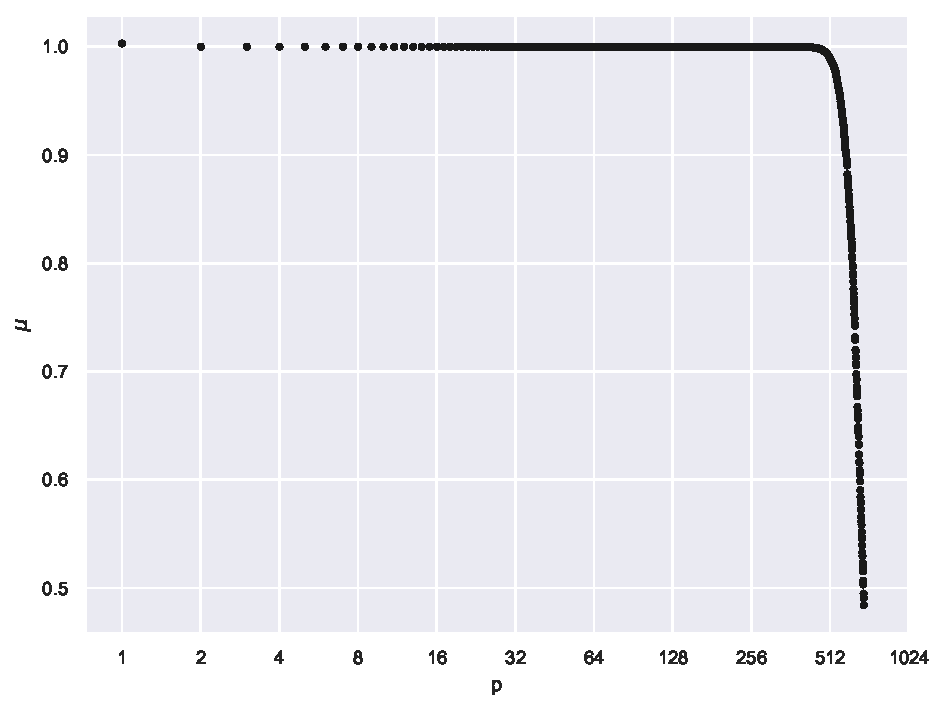
\includegraphics[width=\textwidth]{south_america_eigenvalues_L128.pdf}
	\caption[
		The Slepian eigenvalues of the South America region
	]{
		The ordered eigenvalues of the South America region.
		The majority of the eigenvalues are \(\almost{\num{1}}\) before decreasing rapidly towards zero around the Shannon number \(N=690\).
	}\label{fig:chapter4_eigenvalues}
\end{figure}
